\lhead{\emph{\leftmark}}  
\chapter{The Umplificator Technologies}
\label{chap:tool}
In this chapter, we provide an overview of the tool we have developed to support umplification; as well as discuss some of its technical details including its architecture and a detailed description of the Rule-Engine component. We also present the various design decisions we made as well as the alternatives implementations we attempted during the initial stages of our work. 

\section{The Umplification tool support goals}
In this section, we state what are the desirable aspects for a tool supporting the Umplification process. 

Our objective is to create an accurate tool that can enable developers to efficiently recover the model from existing software systems written in an object-oriented programming language. The Umplificator should provide extensible mechanisms to create and define transformation rules. In fact, the most important goal for a successful reverse engineering environment is that it must provide an extensible toolset \cite{tilley1994programmable}. The extensibility should be present in all the different operations of the tool such as parsing the input source code, transforming the source code and presenting the information. The end-user should be able to provide their own tools for these activities or to extend the ones already provided.  The high-level \textbf{general} and \textbf{specific} requirements for the tool are presented below. General requirements are the ones that every reverse engineering tool should possess and the specific requirements are the ones additionally required to implement the Umplification process (which may differ from other approaches).

\textbf{General Requirements}\\
A reverse engineering tool generally performs operations to gather information from a software system, organizes the information and presents it in manner such that software engineers can better understand the system. In the literature explored in Chapter \ref{chap:related} most of of the tools exhibit a layered architecture with a parser, analyzer and (XMI, XML) code generator as common components.

The general requirements for our specific tool are presented below with an emphasis on the component involved.

\begin{itemize}
\item The tool must be able to \textbf{parse} any of the most popular Object-oriented programming languages.
\item The tool must be able to handle of  the different idioms and programming conventions of those programming languages (parser and analyzer).
\item The tool should be able to \textbf{export} the output in different formats (code generator).
% When you say this it is not clear what formats you mean. You really mean Umple. What else?
\item The tool must offer both GUI and command-line capabilities. Command line capabilities are needed for automated testing, and scripting and for back-ends that permit deployment of the tool on the Web.
\item The tool should support incremental updates of the target model. This is required for large models as the target model does not need to be regenerated completely after each transformation. 
\end{itemize}

% Deleted a block here that was completely duplicated  -- FIXED

\textbf{From the developer's perspective:}
\begin{itemize}
\item The tool should be easy to debug. We should be able to quickly identify the location of an error and fix it.
\item The mapping rules should be as general and extensible as possible. 
\end{itemize}


\section{Alternative Approaches Studied}
We have explored two different and famous model transformation technologies with the purpose of umplifying a software system: TXL \cite{Cordy2006} and ATL \cite{atl}. In the following two sub-sections we present the mapping rules, grammar and program directives that allowed us to transform a Java Program into Umple. 

\subsection{TXL}

TXL \cite{Cordy2006} is a programming and rule-based language and rapid prototype system designed for implementing source transformation tasks. 

The TXL paradigm consists of parsing the input text into a tree according to a specified grammar, transforming the tree to create a new output parse tree and parsing the new tree to finally produce the output text. In TXL, grammars and transformation rules are specified in the TXL programming language. The TXL processor is responsible for interpreting both the grammar and mapping rules by using an internal tree-structured bytecode. TXL programs depend on no other tools or technologies and can run on any platform directly from the command line.
TXL programs are composed of a\textbf{ base grammar}, which specifies the syntactic forms of the input structure, a set of \textbf{grammar overrides}, which extend the grammar to be used and a set of \textbf{transformation rules and functions}, that specify how the input structure will be transformed to produce the desire output structure.

The \textbf{grammar} in TXL is a description of the structure to be transformed in EBNF in a context-free ambiguous form.
% Ambuguous?

The\textbf{mapping rules and functions} specify how to transform the input text into the desired output. The mapping rules are specified using pattern and replacement pairs: 

\vspace{\baselineskip}
\begin{lstlisting}[style=umplePlain]
LeftHSPattern -> RightHSPattern IF Condition
\end{lstlisting}

Where \textit{LeftHSPattern} and \textit{RightHSPattern} are term patterns. The result of a mapping rule is the instantiation of the \textit{RightHSPattern} and is produced when the term matches the \textit{LeftHS\_Pattern} and the condition is true. Rules are applied recursively until they fail. Functions are similar to Rules but they are applied once on the entire function input.

TXL has been used widely in software engineering tasks and other areas including database migrations and artificial intelligence. We present our experiment in building a \textbf{Java-to-Umple} transformer using TXL. We first studied the similarities and differences between Java and Umple and classified the necessary transformations for converting Java programs to Umple into three categories.

The first category represents the direct transformations where one-to-one mapping between the two languages exists and some rules for minor adaptations are required. For instance, a Java class declaration can be written as: 

\vspace{\baselineskip}
\begin{lstlisting}[style=umplePlain]
ClassModifier class Identifier TypeParameter Super Interfaces ClassBody
\end{lstlisting}

In this, the \textit{ClassModifiers} are used to control the access to members of a class, the Identifier specifies the name of a class, the optional \textit{TypeParameter} are used when the class is generic and declares one or more type variables, the Super clause specifies the direct superclasses of the current class, and the Interfaces clause specifies the name of the interfaces that are direct super-interfaces of the class being declared.

Very similarly, an Umple class is defined as: class Identifier \textit{ClassBody}. In this case we will need a mapping rule matching the Identifier and class keyword in the Java program to produce the desired output, the Umple class. 

The second category corresponds to the \textbf{indirect transformations} where some special functions are needed to map a Java construct to an Umple one. For example, a Java instance variable can be mapped to an Umple attribute, an Umple Association or an Umple state machine. This kind of transformations requires helper and additional functions in the TXL program. 

\subsubsection{Java to Umple Implementation}

In this section, we describe the design process. Next, we describe the implementation of the JavaToUmple program that partially converts Java code to Umple. Lastly, we provide examples of transformations rules in the TXL language. Figure \ref{fig:txl} presents the components of the TXL \textbf{JavaToUmple} program. 

\begin{figure}[h]
\centering
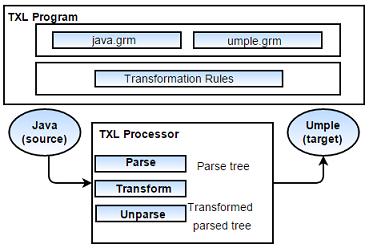
\includegraphics[width=0.75\textwidth]{Figures/TXLprogram.png} 
\caption{TXL Program for transforming Java to Umple}
\label{fig:txl}
\end{figure}

\subsubsection{Design process of the TXL Program}

The first step in writing a source transformer is writing working grammars for both the target and the source language and then writing a union grammar that accepts constructs for both languages. A grammar for Java 1.5 is available from the TXL website [REF]. We wrote the grammar for Umple in EBNF format required by the transformation engine. We then built the TXL rules and functions grouped in modules. Each module targets conversion of one specific language construct of Java to the equivalent in Umple and is stored in a separate file. The overall structure of the transformer is shown in Figure \ref{fig:txlStructure}. It contains the modules for the different language constructs and the main model that starts the program. Below, we briefly describe the different modules:
% ref above

\begin{figure}[h]
\centering
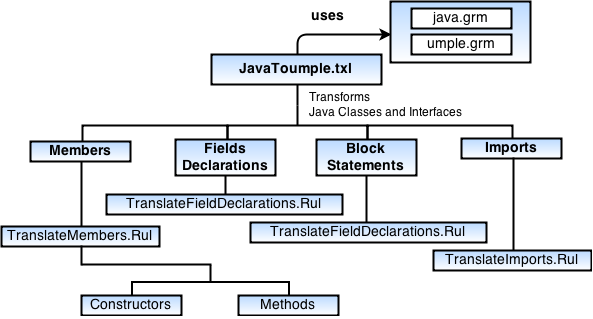
\includegraphics[width=0.98\textwidth]{Figures/TXL_STRUCTURE.png} 
\caption{Structure of the JavaToUmple program}
\label{fig:txlStructure}
\end{figure}

\begin{itemize}
\item JavaToUmple.Txl: This is the main program. It is used by TXL to match an input Java program against the Java Grammar and to call the transformation rules.
\item TranslateMembers.Rul: Contains rules and functions to transform nested declarations.
\item TranslateFieldDeclarations.Rul: Contains rules and functions to transform field declarations.
\item  TranslateBlockStatements.Rul: Contains rules and functions for matching bodies of code belonging to constructors and methods.
\item TranslateImports.Rul: Contains rules for matching Java imports.
\item TranslateConstructors.Rul: transforms the Java constructors.
\item TranslateMethods.Rul: transforms Java Methods.
\end{itemize}

The original Java source code remains untouched after applying the transformation. A set of one or more Umple files is produced as result of the transformation. The \textbf{JavaToUmple} program can be invoked using the command:
%There needs to be some vertical whitespace before listings automatically when the don't have a listing number like here   - FIXED
\vspace{\baselineskip}
\begin{lstlisting}[style=umplePlain]
< txl –o outputFileName.ump inputFileName.Java JavaToUmple.txl >
\end{lstlisting}

\subsubsection{JavaToUmple - Transformations Examples}

In this sub-section we provide some transformation examples. We first show the Java and Umple grammar for the single constructs we transform as well as the TXL transformations rules that guide the transformation.

\textbf{Example 1: Transforming the Class Header} \

In order to transform a Java class into an Umple class, we need to first transform the class header. The code excerpt in Listing \ref{lst:bnftxl} below shows the EBNF grammar for class definitions in both Java and Umple languages. An example of class definitions is also provided in Listing \ref{lst:sampletxl}.

\begin{lstlisting}[style=umplePlain, caption="Class definition grammar in BNF form", label=lst:bnftxl]
JavaClassDeclaration: 
   ClassModifiers? class Identifier Super? Interfaces? ClassBody


UmpleClassDeclaration: 
   class Identifier ClassBody  ClassBody: '{' ClassContents '}'

\end{lstlisting}

\begin{lstlisting}[style=umplePlain, caption=Class definitions in Java and Umple, label=lst:sampletxl]
// In Java:
public class A extends X implements Z {
    //…some contentW
}
// In Umple:
class A 
{	
 //.. some content
}
\end{lstlisting}

The mapping rule called '\textit{changeClassHeader}' that transforms class headers of a Java class is presented below in Listing \ref{lst:classHeader}. In order to transform the class header from Java to Umple, we need to deconstruct the class header  (Line 4)  of a Java class and take only what is required in an Umple header, the identifier of the class. The modifiers of the class are discarded and the extends and implements clauses are ignored at this moment, they are analyzed and transformed in subsequent steps of the program transformation. 

\begin{lstlisting}[style=umplePlain, caption=TXL Mapping rule for transforming the class headers, label=lst:classHeader]
rule  changeClassHeader 	
   replace $[class_header] 		
    	ClassHead[class_header] 		
    	deconstruct ClassHead 					
    	modifiers[repeat modifier] 'class Name[class_name] 
        ExtendClause[opt extends_clause] 
        ImplmntClause[opt implements_clause]          
    by 	 'class Name 
end rule

\end{lstlisting}


A \textbf{package} in Java can be defined as a grouping of related classes (and types). In Umple a \textbf{namespace} allows to group Umple classes. Listings \ref{lst:txlpackage} - \ref{lst:txlpackage2} show the EBNF grammar of package definition in both languages and an example. 
% Listings are not properly referenced above ... appear as question marks

\noindent\begin{minipage}{.45\textwidth}
\begin{lstlisting}[style=umplePlain,caption=Java Package,label=lst:txlpackage]{Name}
PackageDeclaration:
   package PackageName; 


package aPackageName;
\end{lstlisting}
\end{minipage}\hfill
\begin{minipage}{.45\textwidth}
\begin{lstlisting}[style=umplePlain,caption=Umple Namespace,label=lst:txlpackage2]{Name}
PackageDeclaration:
   namespace NamespaceName;
 
namespace aNamespaceName;
\end{lstlisting}
\end{minipage}


The mapping rule called '\textbf{changePackageToNamespace}' that transforms package declarations is presented below:

\begin{lstlisting}[style=umplePlain, label=lst:packageDeclRule, caption=TXL mapping rule for the transformation of the package declaration]
rule changePackageToNamespace 
    replace [opt package_header]      
            'package Name [package_name] '; 
    by       
            'namespace Name '; 
end rule	
\end{lstlisting}

An import declaration in Java allows a named type or a group of named types to be referred to. The '\textbf{Depends}' construct in Umple is similar to this. 

\noindent\begin{minipage}{.45\textwidth}
\begin{lstlisting}[style=umplePlain,caption=Java Import]{Name}
ImportDeclaration:
     import  QualifiedName; 


import java.io.StreamReader;
public class A {
 //…
}
\end{lstlisting}
\end{minipage}\hfill
\begin{minipage}{.45\textwidth}
\begin{lstlisting}[style=umplePlain,caption=Umple Depend]{Name}
DependDeclaration:
   depend QualifiedName;


class A {
  depend java.io.StreamReader;
}
\end{lstlisting}
\end{minipage}

The mapping rule called '\textbf{changeImportToDepend}' that transforms import declarations is presented below: 

\begin{lstlisting}[style=umplePlain, label=lst:packageDeclRule, caption=TXL mapping rule for the transformation of the import declaration] 
changeImportToDepend  	
    replace [repeat import_declaration]      
           'import Name [imported_name] '; 
    by 	   'depend Name '; 
end rule
\end{lstlisting}

As seen in the example, the depend declarations appear inside the Umple class, so we need additional rules to remove them from the top of the Java class and place them in the right place when the Umple code is generated. The rule below removes all the import declarations. The main program, presented next, illustrates how the program executes the mapping rules in order to produce the output.

\begin{lstlisting}[style=umplePlain, label=lst:packageDeclRule, caption=Helper Function used to remove the imports declarations] 
function removeImports  
    replace * [package_declaration]
        PkgHead [opt package_header]   
        ImpDecl [repeat import_declaration]  
        TypeDecl [repeat type_declaration] 
    by   
        PkgHead      TypeDecl
end function
\end{lstlisting}

The main program in Listing \ref{lst:mainProgramtxl} is used to execute the three mapping rules presented in the examples above; it calls one by one the rules and the functions and generates the output. Additionally, the main program links (via inclusion constructs) the grammars from the target and source languages. In the \textbf{JavaToUmple} program we use two grammar files to map Java and Umple constructs: \textit{Java.GRM} and\textit{ Umple.GRM}.

\begin{lstlisting}[style=umplePlain, label=lst:mainProgramtxl, caption=The ATL main program - JavaToUmple.Txl] 

include "java.Grm" 
include "Umple.Grm" 

function main    
    replace [program]
        P [program]     
    by 	P [javaToUmple]
end function 

function javaToUmple   
    replace [program] 
         P [program]     
    by 
        P 
        [changePackageToNamespace] 
        [changeImportToDepend] 
        [removeImports] 
        [changeClassHeader]
end function 
% ****	MAPPING RULES HERE   ****
\end{lstlisting}

The transformation program above uses the two grammar files to map Java and Umple constructs:  java.GRM and Umple.GRM. The program rules have been modularized for a better understanding as it has been shown in Figure \ref{fig:txlStructure}.

\subsection{ATL}

ATL (ATL Transformation Language) \cite{atl} is a model transformation language that provides ways to produce a set of target models from a set of source models and allows users to define model-to-model transformations in both a declarative and imperative way.
ATL has been developed in Eclipse as a set of plug-ins by the Institut National de Recherche en Informatique et en Automatique (INRIA) as an answer to the Object Management Group's QVT language request for proposals [REF].  The ATL environment in Eclipse offers an ATL editor with syntax highlighting and code completion capabilities, a debugger and a profiler that aims to ease the development and testing of model transformations.
% Missing reference above --FIXED

In this section, we describe how queries, views and transformations are handled in ATL. Additionally, we explore the ATL transformations required to umplify a Java system. Figure \ref{fig:atl} presents the core idea behind an ATL transformation.

\begin{figure}[h]
\centering
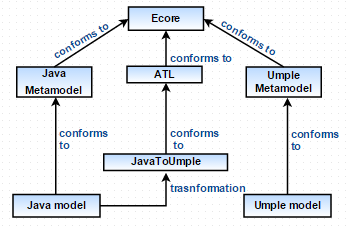
\includegraphics[width=0.75\textwidth]{Figures/ATL_PROGRAM.png} 
\caption{The JavaToUmple ATL program}
\label{fig:atl}
\end{figure}
%The figure is not pretty. Can you reduce the font size and avoid all capital letters? When I look back, I see a similar thing in Figure 5.1, although the text is not so large. Text in figures should be not much larger than text in the main body

\subsubsection{The basics of ATL}

The ATL language is composed of expressions to query model elements (queries), views to handle incremental transformations and transformation rules to direct the transformations of  a set of source models to a set of target models.

\textbf{Queries}

A query in ATL is an expressions allowing one to search and return model elements from a model defined in an OMG-compliant format. A query is an OCL expression that can return primitive values, model elements or a combination of these. A query can’t alter the source model. It is possible to navigate across model elements and call query operations on these. For instance, when the following query is executed on a Java model, it first gets the set of all existing JavaElement classes in the model and gets the size of the computed set. The computed integer value is cast into a string before being written into the file 'metrics.txt'. 

\vspace{\baselineskip}
\begin{lstlisting}[style=umplePlain]
query JavaElementNb  =
  JavaModel!JavaElement.allInstances()->size().toString()
       .writeTo(‘metrics.txt’)
\end{lstlisting}


\textbf{View}
Views in the ATL world are a special case of transformation. Views offer support for incremental transformations. The user can query a model; perform a transformation on a subset of the source model and save results on a view. Then, she can update the view from its source without executing the whole transformation again. 

\textbf{Transformation Rules
}
There are different kind of rules in ATL based on the way they are called and how they specify the results: matched rules, lazy rules and called rules.

\begin{itemize}
\item \textbf{Matched Rules}: 	This kind of rule specifies which source element is to be matched, along with the target element that is to be produced.
\item \textbf{Lazy Rules}: This kind of rule is similar to a matched rule, but it is not executed when matched; they rely on being called by other rules.
\item \textbf{Called Rules:}	This kind of rule can have parameters and can be called only from imperative code.
\end{itemize}

\subsubsection{ATL Tool Support – Eclipse M2M}
%The long-dash above doesn't appear in the output
The ATL project is composed of four parts (or four different plug-ins in Eclipse). The Core, Compiler, Parser and the Virtual Machine (VM), which are described below:

\begin{itemize}
\item \textbf{Core} - Contains the classes used to internally represent a model, to allow the creation of models and metamodels, to save and load models and to supply ways to launch the model transformations. 
\item \textbf{Compiler} - Uses the ACG (ATL VM code generator) domain-specific language to compile and generate code. 
\item \textbf{Parser} -Contains all classes to parse an ATL transformation input and to generate an output model compliant with the target metamodel.
\item \textbf{VM} - A byte-code interpreter.
\end{itemize}

% I think here you ought to discuss the CDT approach (at least give the sort of background you gave for TXL and ATL) without explaining in detail how you used it.

\section{Discussion}

% Here you need to explain the issues you had with TXL and ATL.This should be at least two pages. There should be a table showing comparisons between TXL, ATL and CDT, and a conclusion about why you chose the latter. Stopping for the day.

\section{The Umplificator}
\label{chap:tool}
In this section, we provide an overview of the tool we have developed to support umplification; as well as discuss some of its technical details.
Our tool is called the Umplificator.

The Umplificator takes as input  a set of files containing classes written in base language code (Java, C++ etc.), Umple files, source code directories or software projects (source code containers as represented in many popular IDEs such as Eclipse). The output is an Umple textual model containing base language code with modeling abstractions. 
%DELETE The Umple model is fully compatible with many UML and XMI formats and can be viewed or edited diagrammatically. 
%I suggest deleting this. I assume you have a decent discussion of Umple earlier.

At its core, the Umplificator is a language interpreter and static analyzer that parses base language and Umple code/models, populates a concrete syntax graph of the code/model in memory (JavaModel, CPPModel), performs model transformation on the base language representation in memory and then outputs Umple textual models.

The Umplificator relies on initial parsing by tools such as the Java Development Tool (JDT) for Java, CDT for C++, and PDT for PHP. These extract the input model from base language code. The use of JDT and its siblings reduces the need to write an intermediate parser for the base language.

The base language model is then transformed in a series of steps into an Umple model. To do this, the Umplificator uses a predefined set of refactoring rules written in the Drools rule language \cite{Drools_Book}. Drools is a rule management system with a forward- and backward-chaining rules engine. The rule engine is explored in more detail in Section 4.2.
% TO BE FIXED
%REally 4.2? I assume this is supposed to be a forward reference. If in fact you have already discussed it, then don't introduce it again in the above paragraph.

The Umplificator includes other subsidiary and internal tools such as:
\begin{itemize}
\item Language validators – A set of base language validators allowing validation of the base language code that is generated after compilation of the recovered Umple models.
\item Umplificator statistics –  A metrics-gathering tool to analyze certain aspects of a software system such as the number of classes and interfaces, the  number of variables present in the code, the cyclomatic complexity, the number of lines of code \cite{MetricsBuse}.  
\item Umplificator Workflow – A tool that guides the umplification process within Eclipse.
\end{itemize}
The Umplificator is available as an IDE and works within Eclipse; it also operates as a command-line tool to allow rapid bulk umplification and easier automated testing. Both tools are built and deployed using the Ant scripting language; resulting in several executable jars as well as for the Eclipse plugins. 
The development of the Umplificator follows a test-driven approach to provide confidence that future enhancements will not regress previously functioning and tested aspect of the system. 

\section{Architecture}
The Umplificator has a layered and pipelined architecture. The pipelines (components) in this architectural style are arranged so that the output of each element is the input of the next.  Figure \ref{fig:architecture} presents the architecture.
The process of umplifying a system in this architecture is described below (Figure   \ref{fig:process_flow}). 
\begin{enumerate}
\item The input is a set of source code files in the base language and/or Umple.
\item The source code is transformed into base-a model of the base language and Umple constructs.
\item The model previously obtained is entered into the next stage of the pipeline. The input model is transformed a model with additional Umple features using pre-defined mapping rules. 
\item The target Umple model, is then validated. 
\end{enumerate}

\begin{figure}[h]
\centering
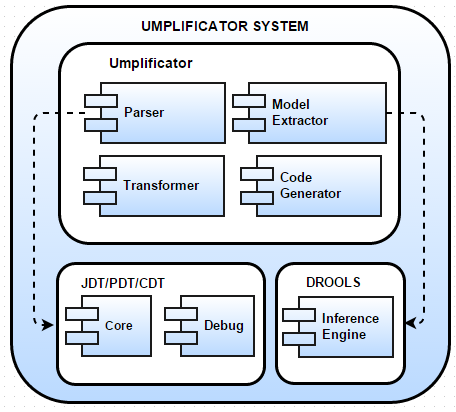
\includegraphics[width=0.75\textwidth]{Figures/UmplificatorComponents.png} 
\caption{The Umplificator components}
\label{fig:architecture}
\end{figure}

The mapping rules and rule engine are introduced in the following sub-section. 

\begin{figure}[h]
\centering
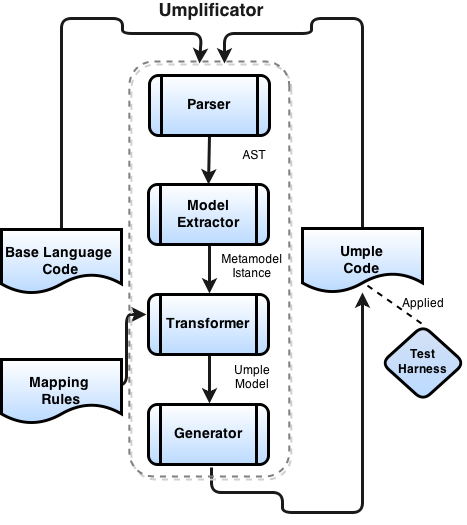
\includegraphics[width=0.75\textwidth]{Figures/Umplificator_ProcessFlow.png} 
\caption{The umplification process flow}
\label{fig:process_flow}
\end{figure}

\subsection{Rule Based Language}
The rule engine interprets and executes the mapping rules on the source model and target model to produce the umplified version of the target model.
The Drools engine used by the Umplificator is composed of an inference engine that is able to scale to a large number of rules and facts.  The inference component matches facts and data (base language models) against rules to infer conclusions, which result in actions (model transformations). A rule is a two-part structure (LHS and RHS) using first order logic for reasoning over knowledge representation. Pattern matching is performed to match facts against rules and is implemented using the Rete algorithm [15]. The rule engine is initialized with the rules. A Drools rule has the basic form: 

\begin{lstlisting}[language={drools},label={lst:drools}, caption=Basic rule in Drools] 
rule "name" 
  when LHS then RHS
end
\end{lstlisting}


where LHS is the conditional part of the rule and RHS is a block that allows dialect-specific semantic code to be executed. 
The rules are grouped in files for each of the cases (levels of refactoring) discussed earlier. In other words, there is a rule file containing rules, functions and queries to transform variables into attributes, another file containing those to transform variables into associations and so on. 
The rules as explained in this paper are instructions indicating how a piece of the Base language model (Java Model, C++ model, etc.) is mapped to a piece of an Umple model. Additionally, in Drools, one can specify:
\begin{itemize}
\item \textbf{Functions}: These are used for invoking actions on the consequence (then) part of the rule, especially if that particular action is used over and over again. In the Umplificator, functions are used instead of helper classes so the logic is kept in one place.
\item \textbf{Queries}: These provide a means to search working memory and store the results under a named value. In the Umplificator, they are used to gather metric information about the models analyzed. For instance, a query numberOfPublicMethods(..) returns the number of methods having 'public' as modifier. Queries do not have side effects, meaning that their evaluation cannot alter the state of the corresponding executing unit. 
\end{itemize}

In the Umplificator, the logic used for model transformations resides in the rules. Moreover, by using rules, we have a single point of truth, a centralized repository of knowledge. Rules can be also read and understood easily, so they can also serve as documentation.
Traditionally, rule engines have two methods of execution [16]: forward chaining and backward chaining. In forward chaining, the facts are asserted into working memory resulting in one or more rules being concurrently true and scheduled for execution. In backward chaining (goal driven), one starts with a conclusion, which the engine tries to satisfy. Drools is a Hybrid Chaining System because it implements both forward and back-ward mechanism. Our Umplificator uses the forward chaining method of operation in which the inference engine starts with facts, propagates through the rules, and produces a conclusion (e.g. a refactoring).  


As an example, consider the rules in Listing . The rule named transformImport(Lines 1-10) matches and converts any Import Declaration (Java Language) into an Umple depend construct. The dependency (Line 8) is then added to a matched Umple Class. The Umple Class is then put into the working memory (Line 9) so subsequent transformations can be made on the object (forward chaining). The rule named JavaFieldIsUmpleAttribute converts Java fields into basic Umple attributes. The attribute is then added to a matched Umple Class (Line 24). The attribute is put into the working memory (Line 25) so subsequent transformations can be made such as determining if the attribute is lazy or not. The rule named isLazyAttribute, not shown here, is used for this purpose. This rule matches and converts any basic attribute (in memory) that conforms to the required conditions into a lazy attribute (e.g. attribute.setIsLazy(true)). The complete set of mapping rules for the umplificator can be found at the umple code repository \cite{MappingRules_Repository}.

\begin{lstlisting}[language={drools},label={lst:rule_import}, caption=Initial Refactoring Mapping Rules]
 rule  "transform_Import"
 when
  import: ImportDeclaration();
  uClass: UmpleClass() ;
 then
  Depend depend = new Depend(getImportName(import));
  uClass.addDepend(depend);
  insert(uClass);
end
\end{lstlisting}


\begin{figure}[h]
\centering
\frame{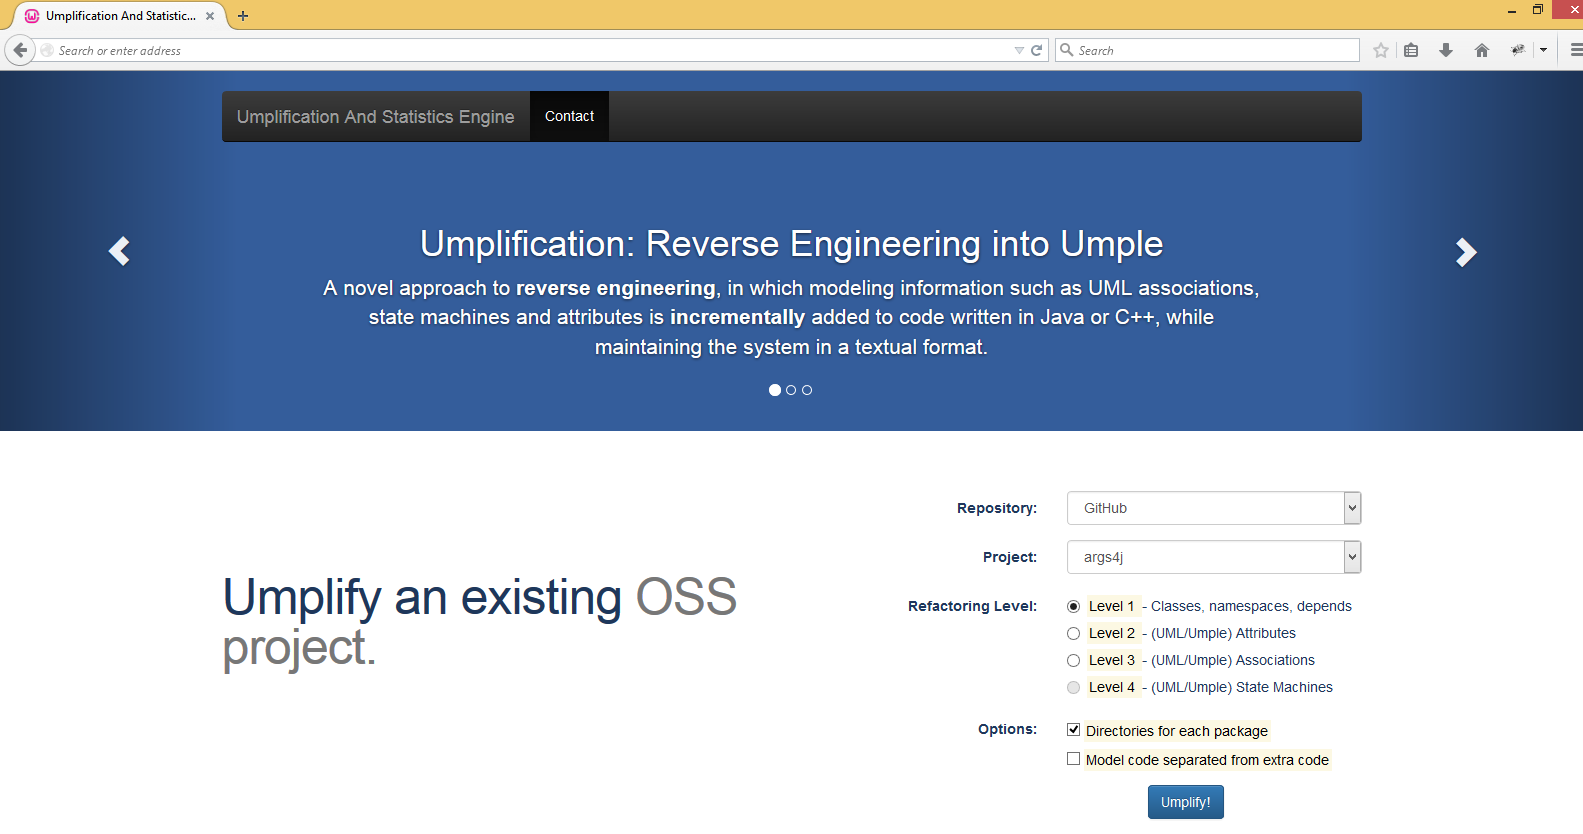
\includegraphics[width=0.98\textwidth]{Figures/UmplificatorOnline.png}}
\caption{The Umplificator online - A PHP Web application}
\label{fig:architecture}
\end{figure}


